
\chapter{Data}

\label{sec:Data Acquisition}
\section{Acquisition}

The data used in this thesis was collected from the W7-X. However, many of the experiments conducted at W7-X won't produce data relevant to the goals of the thesis because due to technical problems, the plasma discharges could not be carried out as planned. Runs (or programs), were carefully selected to include stable plasma conditions. The data was collected from the thermal cameras, which are positioned to take images of the divertor surface of the W7-X (see fig. \ref{fig:data:cameras}). The thermal cameras are used to measure the heat load on the divertor, which is a measure of the amount of heat deposited on the divertor by the plasma. The surface of the the non-planner divertor surface is mapped to a 2-dimensional array of pixel values where each pixel represents the intensity as measured by the thermal camera (see fig. \ref{fig:data:mapping}). The pixel values are then converted to a temperature value using a calibration curve. The temperature values are then integrated over the entire image to give the integrated heat load, $\bar{\iota}$, which is the heat load per unit area. The integrated heat load is the value that is used to train the neural network.

\begin{figure}[htb]
	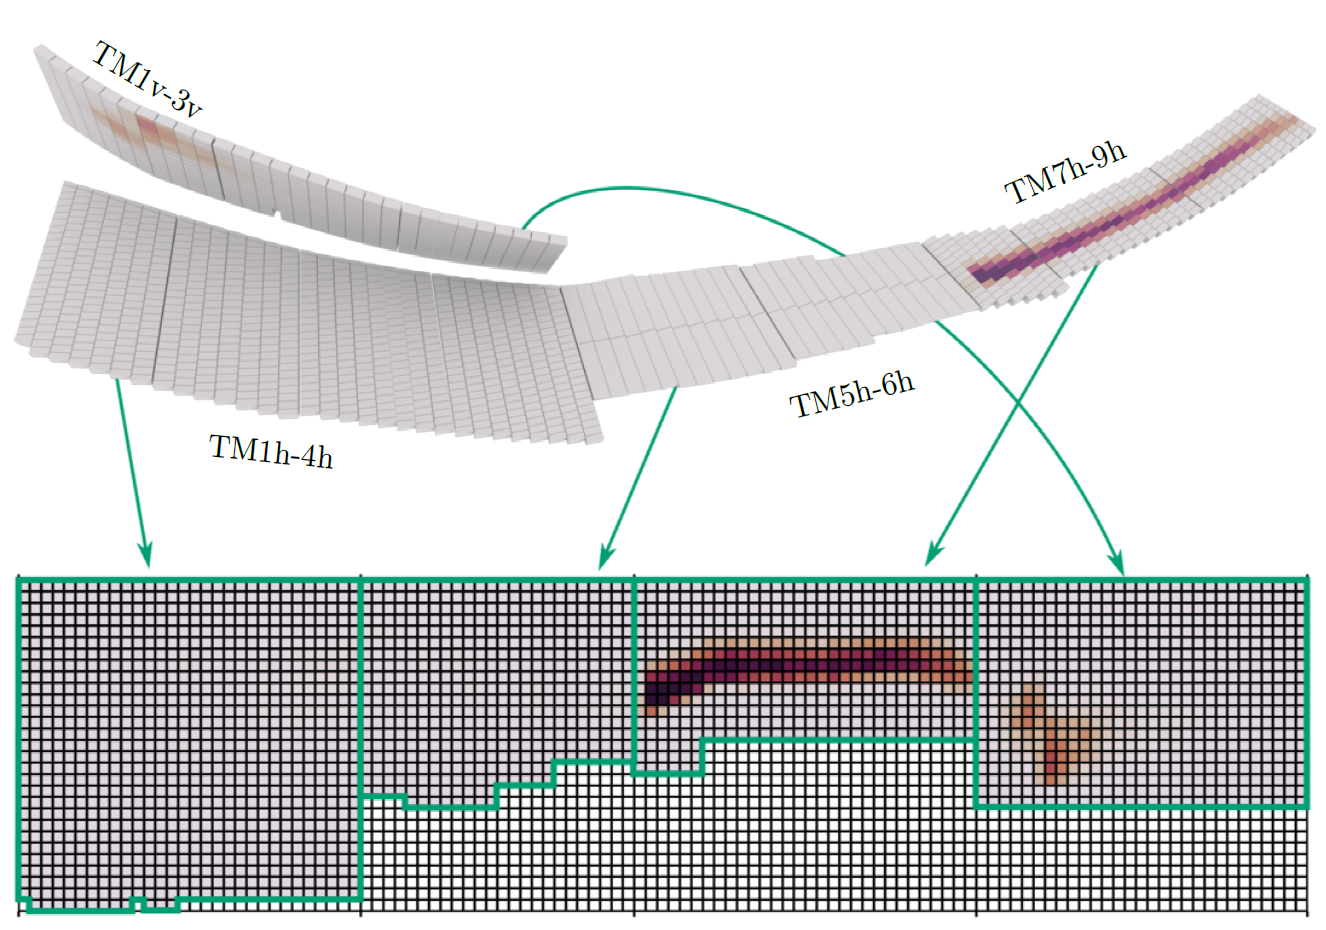
\includegraphics[width=\textwidth]{images/mapping.png}
	\caption{Simulated heat load pattern mapped to a heat load image in arbitrary units. While this case is simulated, the mapping is the same for the experimental data. Image source \cite{Blatzheim_2019}}
	\label{fig:data:mapping}
\end{figure}

\begin{figure}[htb]
	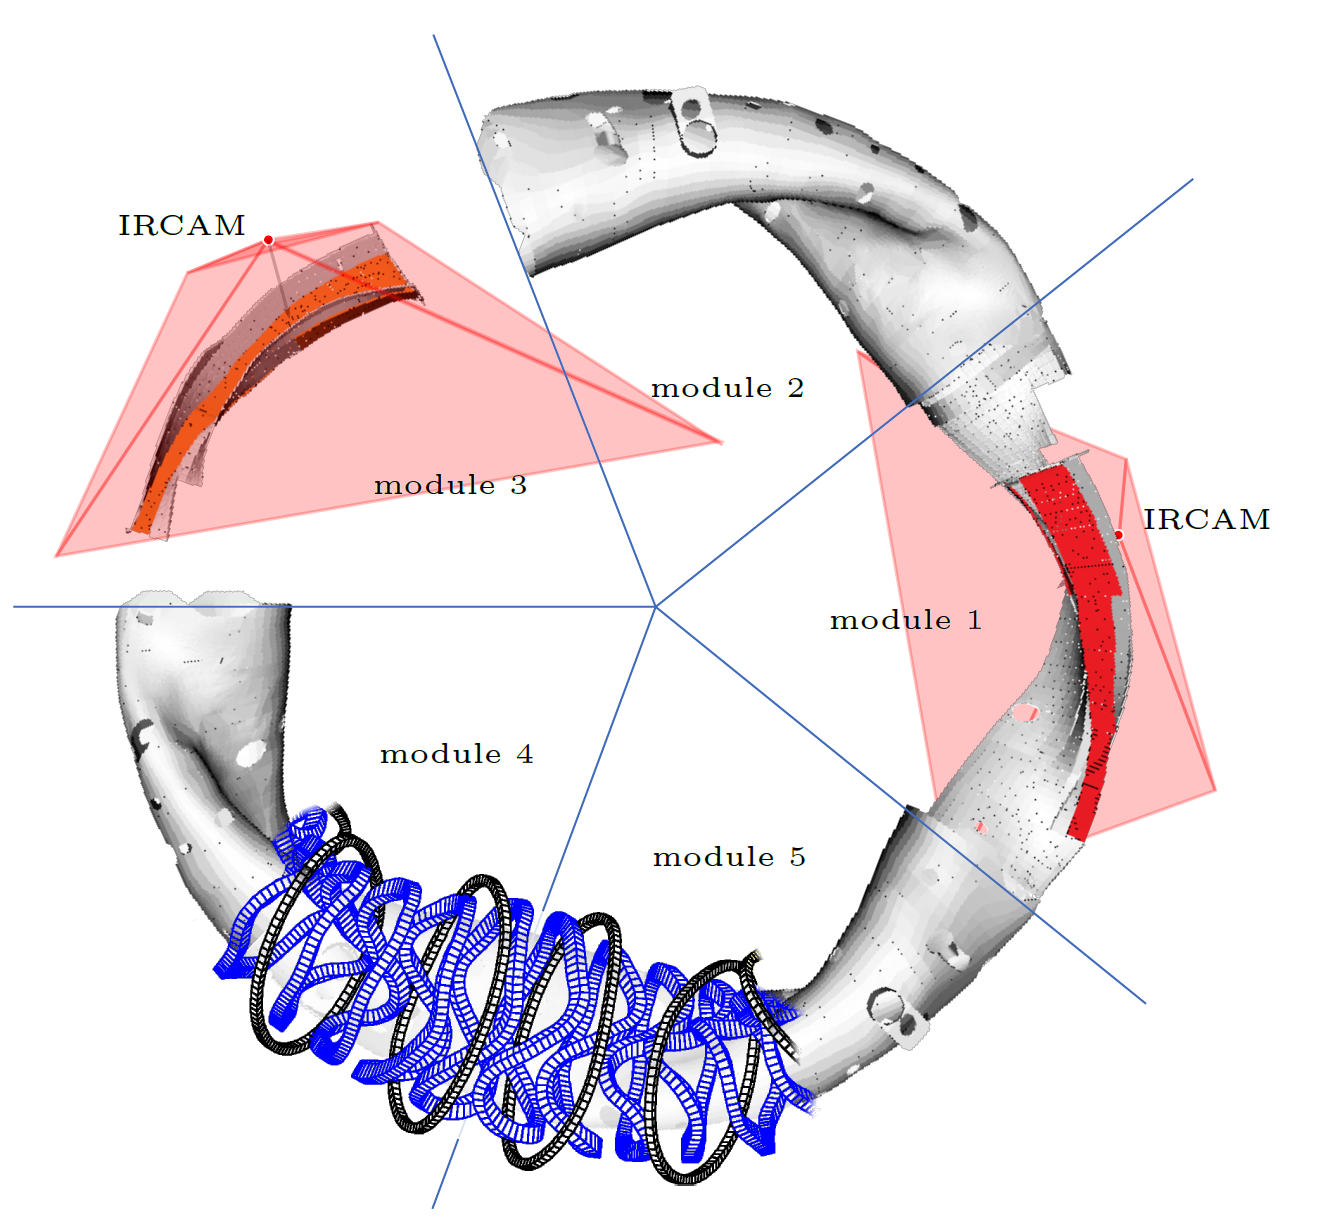
\includegraphics[width=\textwidth]{images/cameras.png}
	\caption{Heat load camera locations and orientations. Image source \cite{Blatzheim_2019}}
	\label{fig:data:cameras}
\end{figure}

\label{sec:Data Selection}
\section{Selection}

Since a program covers several minutes of data collection, the images can exhibit a wide range of heat load patters and many samples my be unsuitable for training. For example, fig. \ref{fig:data:heat_load1} is an example of two heat load images from different timestamps, one early in the experiment and one later in the experiment with higher integrated heat load. The experimental conditions are low $\bar{\iota}$, high heating power, and a low density plasma. Fig. \ref{fig:data:heat_load2} is again two heat load images from different timestamps, this time both from program number 20180927.18, which had high $\bar{\iota}$, low heating power and high density. While the later timestamps for both set of images look dramatically different, with visible heat load patterns and different intensities, the early timestamp images for both pairs are visually indistinguishable. The plasma in the in both early examples had yet to deposit enough heat on the divertor to be resolved by the thermal cameras.

\begin{figure}[htb]
	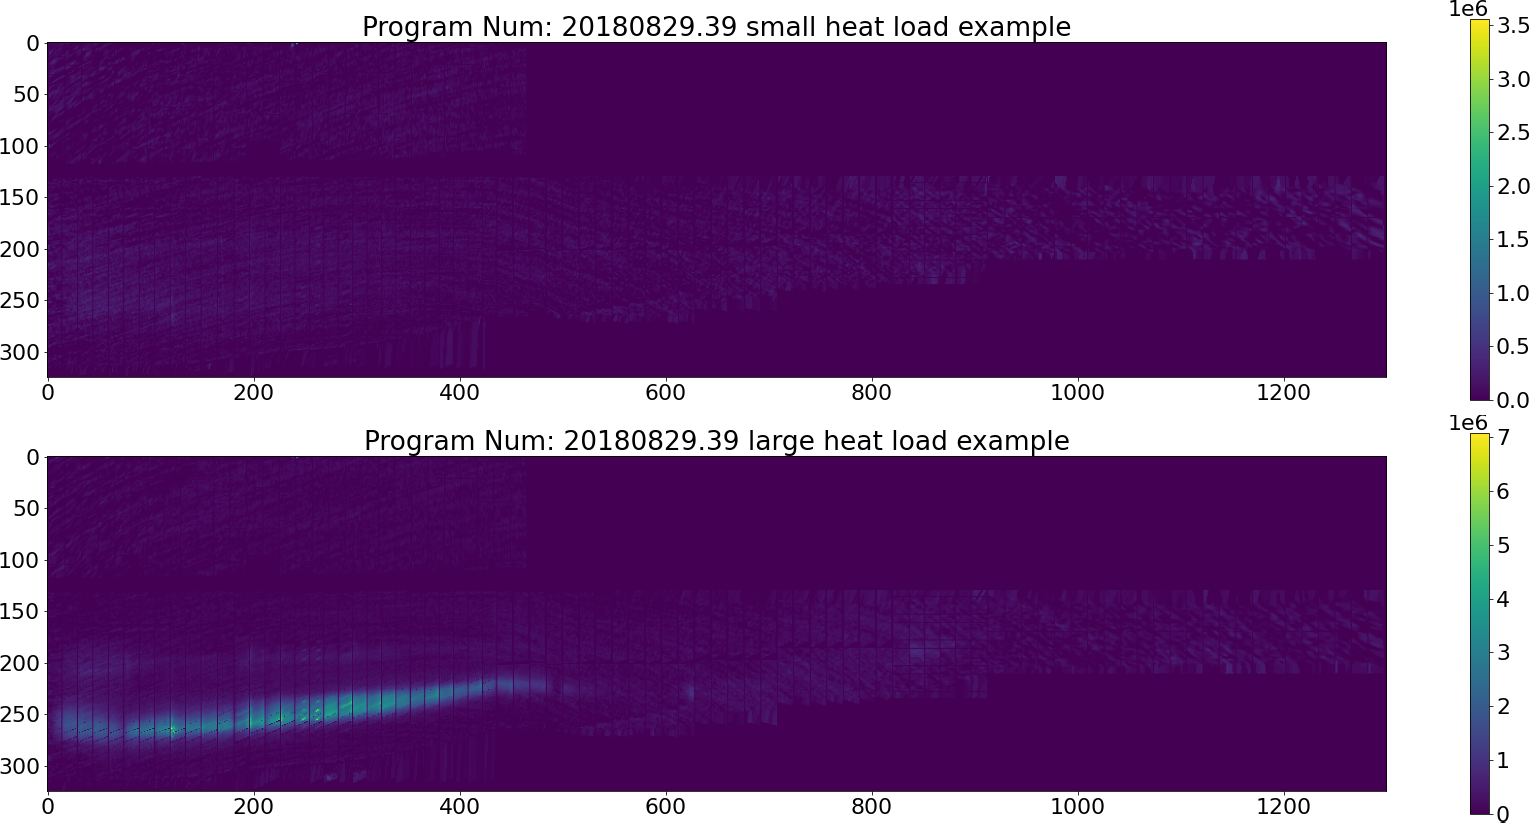
\includegraphics[width=\textwidth]{images/heat_load1.png}
	\caption{An example heat load image. Experimental conditions: low $\bar{\iota}$, high heating power, low density}
	\label{fig:data:heat_load1}
\end{figure}

\begin{figure}[htb]
	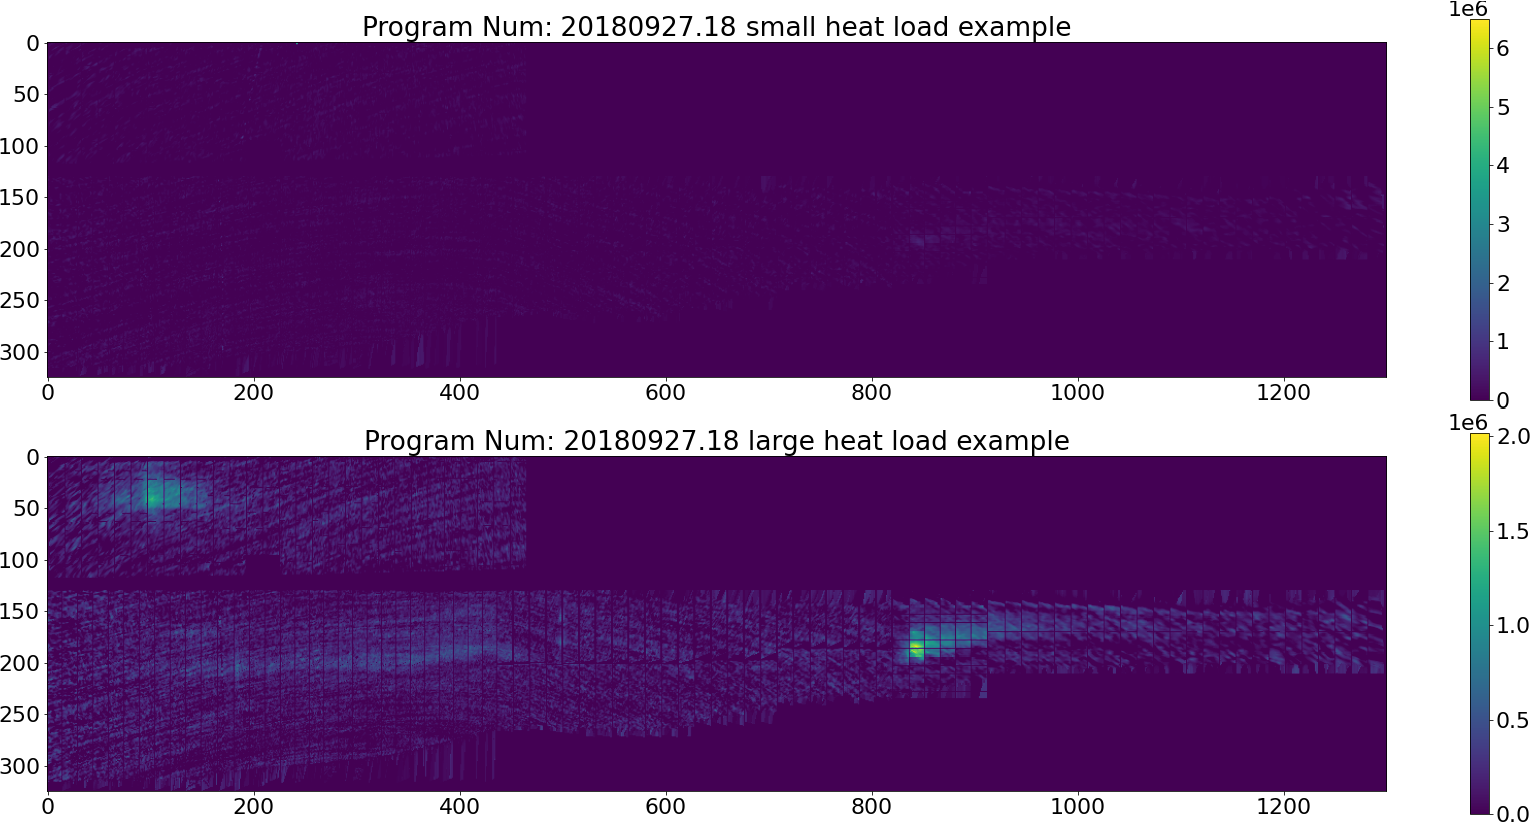
\includegraphics[width=\textwidth]{images/heat_load2.png}
	\caption{An example heat load image. Experimental conditions: high $\bar{\iota}$, low heating power, high density}
	\label{fig:data:heat_load2}
\end{figure}

To filter the unsuitable images, a variety edge cases were hand picked, both unsuitable and suitable examples. The edge cases were then used to create a filter that was applied to the data set. The first attempt at a filter was integrated heat load but the baseline noise levels varied greatly from run to run so it was ineffective. Even setting a threshold for the pixels prior to integrating was ineffective because of the variance in the run to run noise. After some trial and error, the filter that was the most effective is a 24x24 2-dimensional convolutional kernel of ones (a 24x24 matrix of ones) to the image, effectively summing the values in a 24x24 pixel window to a single pixel. The filter this size would help dilute anomalous high pixel values in the data but visible signals, which were more spatially localized than the noise, stood out more. The convolved pixels that were dominated by noise were then filtered using a threshold and the heat load from the unfiltered pixes was integrated. The resulting images were then used to train the network. The two threshold values were selected to keep as much suitable data as possible while excluding as much unsuitable data as possible. The thresholds and convolutional kernel size were hand tuned but could be automated by using a grid search to find the optimal values in the future. Since the amount of data included or excluded by this process was not significant, the hand tuned values were used as they were easier to implement.




\label{sec:Data Simulation}
\section{Simulation}

The $\bar{\iota}$ values used for training (training labels) were simulated using the VMEC \cite{VMEC}, a package included in larger package of simulation tools used for optimizing stellarator designs \cite{STELLOPT}. VMEC uses a variational method to solve the toroidal equilibrium equations for a stellarator, minimizing the total energy of the system\cite{VMEC}. To run the simulation, the same experimental conditions were used for a given heat load image.

\label{sec:Data Distribution}
\section{Distribution}

Since the heat load image data was taken from real experiments, the data set is not uniform in the distribution of $\bar{\iota}$ values, which is shown in figure \ref{fig:data:iota_dist}. This means the distribution the network is attempting to learn is nonuniform, or more explicitly, it's multimodal. This is a common problem in machine learning and is often addressed by using a loss function that is robust to multimodal distributions. The loss function used in this case is the $rmse$ \ref{eq:rmse}. The $rmse$ is a common loss function for regression problems, but it is not entirely robust to multimodal distributions. This was address by M. Blatzheim et al.\cite{Blatzheim_2018} by using simulated input data that provided a continuos extension to the output distribution.

\begin{figure}[htb]
	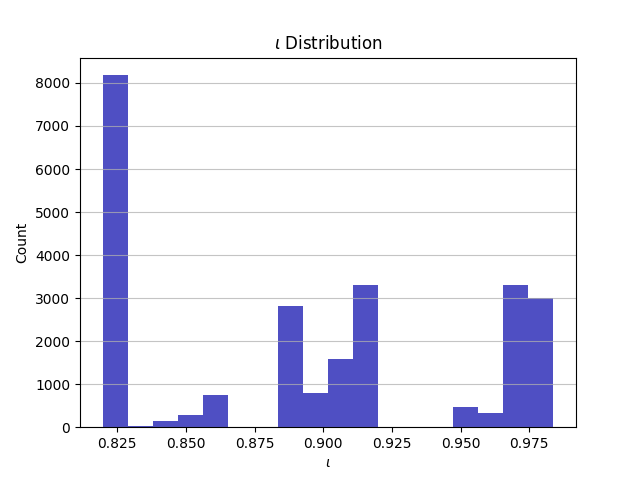
\includegraphics[width=\textwidth]{images/iota-dist.png}
	\caption{Distribution of simulated $\bar{\iota}$ values in the data set.}
	\label{fig:data:iota_dist}
\end{figure}

In an attempt to resolve the imbalanced distributions of the training, validation, and test sets were chosen to be as uniform as possible. This was challenging because the data is broken up into 42 different program numbers. Each program numbers will have highly correlated data so mixing data from program numbers that are included in the test and validation set could serve to pollute the metrics used to evaluate overfitting or hyperparameter tuning. Overfitting occurs when the model learns patterns in the training data that do not generalize to new data, leading to poor performance on the validation or test set. Since the training set requires the most data, the remaining test and validation sets cannot include more than a few runs.

